\subsection{Conversion spectra to the cross section}

\begin{figure}[htbp]
  \centering
  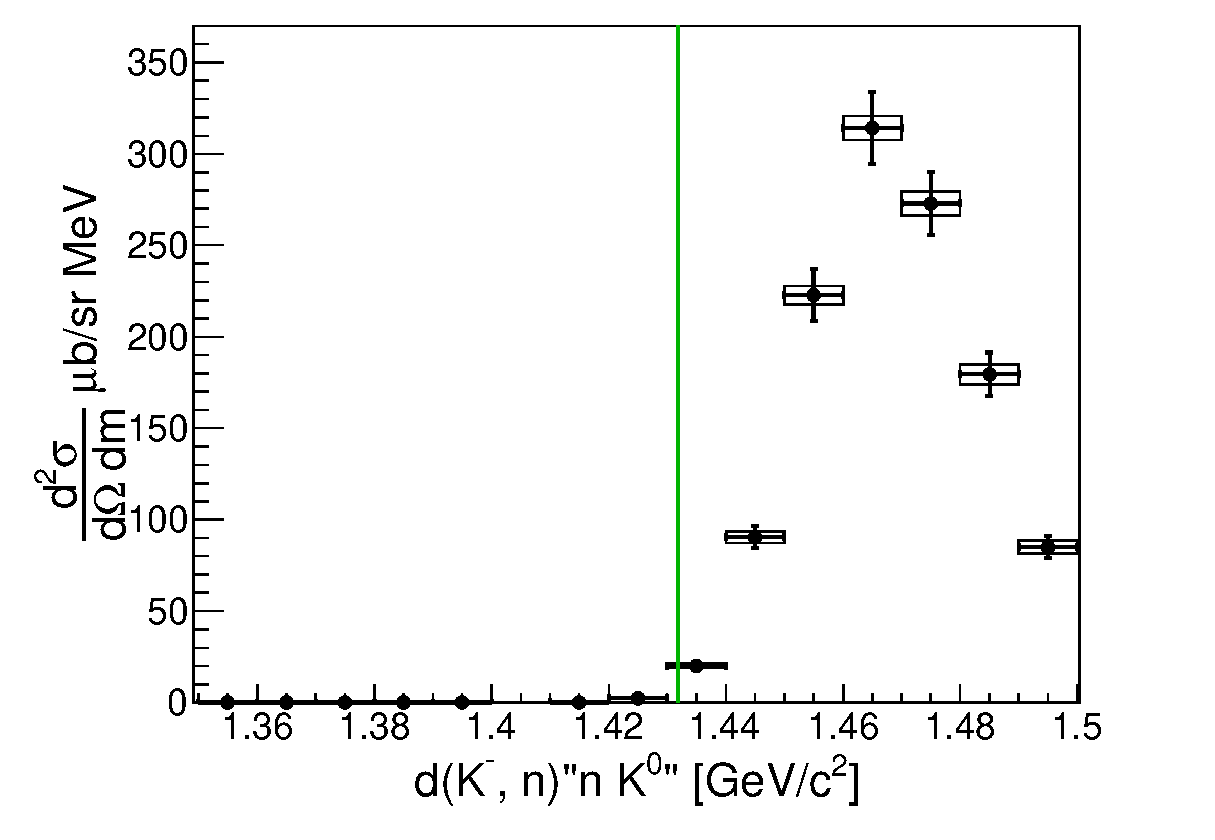
\includegraphics[width=6cm]{../pic/Dron/K0_ana/K0_CS.eps}
  \caption{
    This figure shows the cross section of $d(K^-, n)"n K^0"$.
    The box represents the statistical error, and the error bar represents the root mean squares of the conversion factor added to it.
    The green vertical lines indicates $\bar{K}N$ threshold.
  }
  \label{fig:nK0_CS}
\end{figure}

\begin{figure}[htbp]
  \centering
  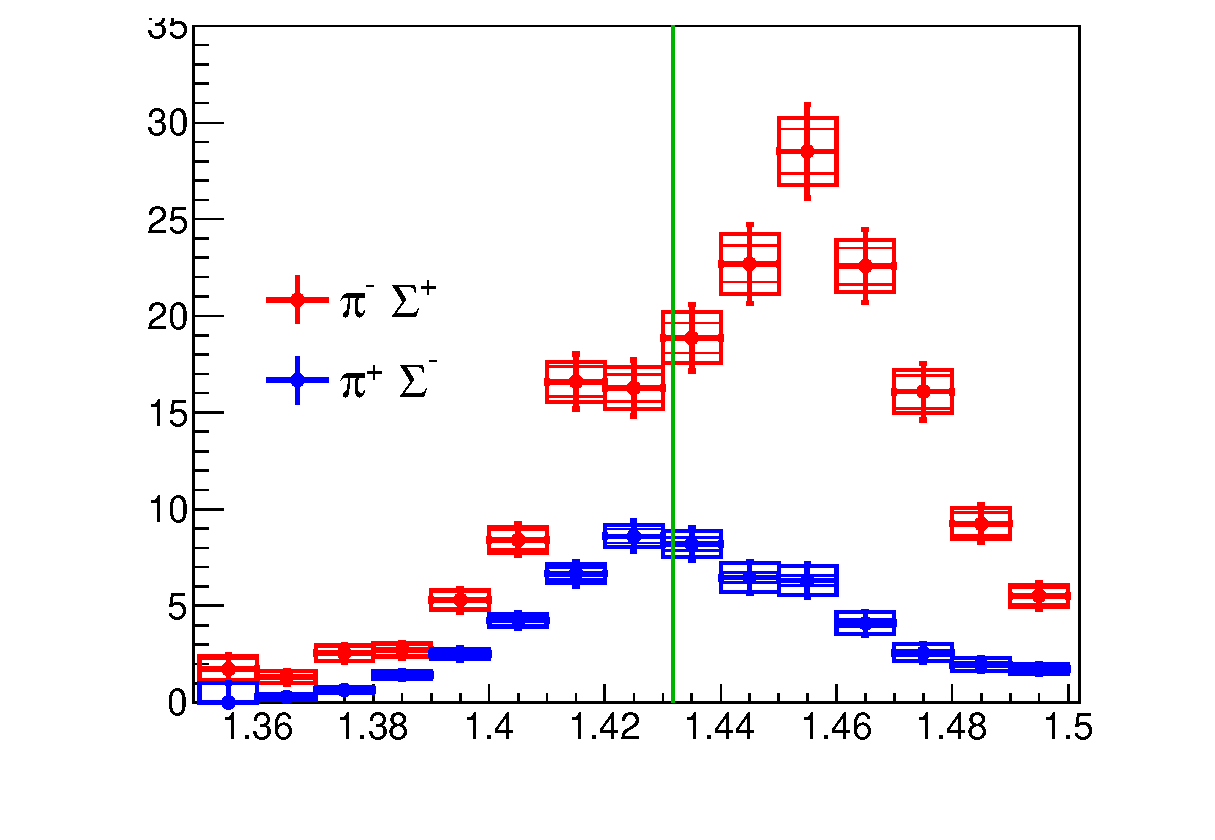
\includegraphics[width=6cm]{../pic/Dron/KN_ana/ChargeCS.eps}
  \caption{
    The red figure and blue figure shows about $d(K^-, n)"\pi^+\Sigma^-"$ and $d(K^-, n)"\pi^-\Sigma^+"$, respectively.
    The inner frame (thin line), outer frame (thick line), and error bars represent the addition of statistical errors, fitting errors, and conversion errors, which were calculated by root-mean-square.
    The green vertical lines indicates $\bar{K}N$ threshold.
  }
  \label{fig:ChargeCS}
\end{figure}

\begin{figure}[htbp]
  \centering
  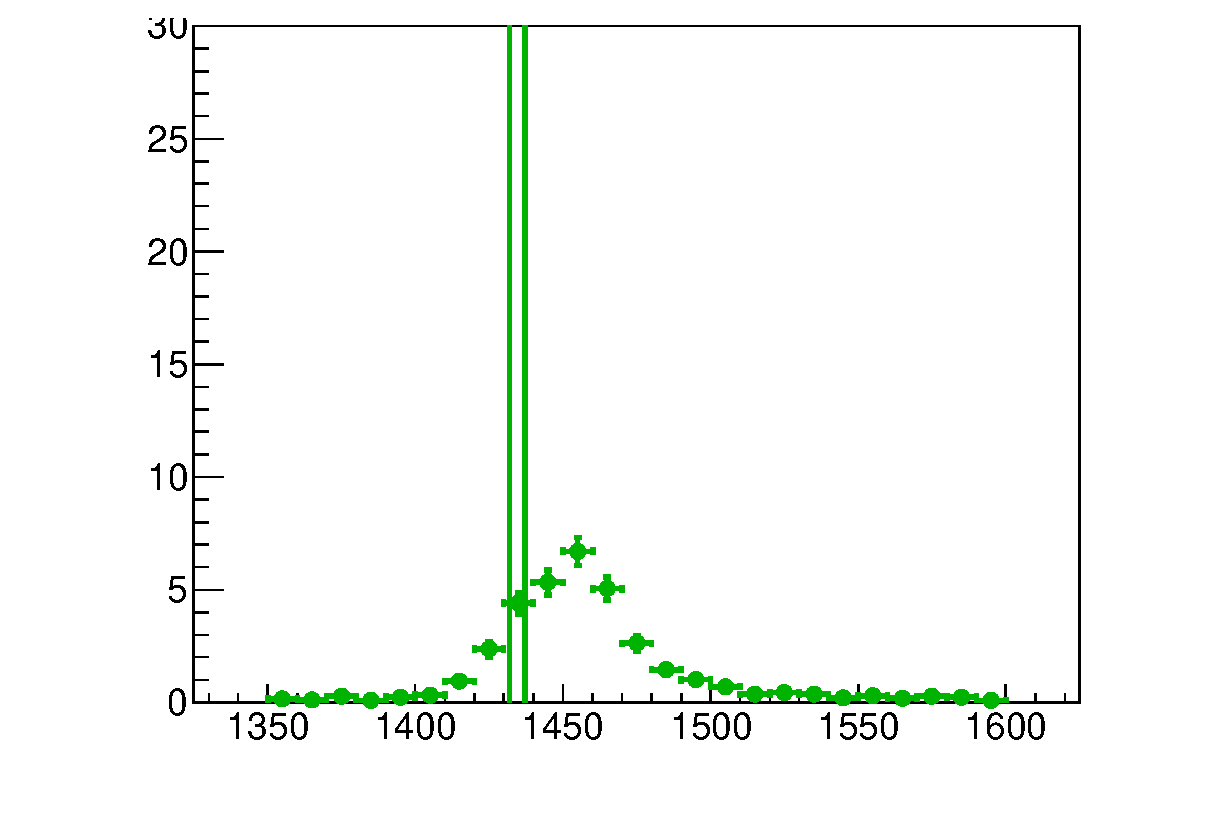
\includegraphics[width=6cm]{../pic/Dron/KP_ana/pimS0_CS.eps}
  \caption{
    This figure shows the cross section of $d(K^-, p)"\pi^- \Sigma^0"$.
    The box represents the statistical error, and the error bar represents the root mean squares of the conversion factor added to it.
    The green vertical lines indicates $\bar{K}N$ threshold.
  }
  \label{fig:pimS0_CS}
\end{figure}

\subsection{$d(K^-, n)$ scaling factor}
$d(K^-, n)"X"$ spectrum can be converted from counts to the differential cross section ($\frac{d^2\sigma}{d\Omega dm}$) excepting the acceptance of the the CDS that is depend on the reaction.
The parameters was used for the conversion were summarized in Table\ref{tab:KN_scale}.

First one is luminosity which was consist of number of target, number of irradiated kaon, DAQ live rate, trigger efficeincy.
The number of target was defined from length of fiducial volume ($10cm$) and target density which was evaluated from measured tempature.
The number of irradiated kaon was defined by correcting kaon number counted up by the scaler DAQ by ratio of true kaon in kaon trigger which was described in Sec\ref{sec:beam_line_ana}.
About DAQ live rate and trigger efficiency were discribed in Sec\ref{sec:trigger}.
The luminosity was evaluated run-by-run.
In the table, these items were represented value weighted by data statistics as typical value.

Next is about the CDS which was CDC efficiency discribed in Sec\ref{sec:CDC_eff}.
Accpectances of CDS were estimated and corrected by the Monte Carlo simulation data.
These evaluations were described in individual section for each reactions.

Last one is about the NC which was consists of acceptance and efficiency.
The efficiency of the NC was further decomposed to intrinsic one and overveto by the CVC and the BVC that was described in Sec\ref{sec:NC_eff}.
The acceptance of the NC was estimated from the NC position and the error was evaluated from difference of the first layer and the last layer of the NC.

\input{analysis/KN_scaling_table}


\begin{table}
  \caption{
    Summary table of $d(K^-, p)$ scaling parameters
  }

  \hspace{-2cm}
  \begin{tabular}{cc|cc|cc}
    \multicolumn{2}{c|}{Component}  & value            & error           & value  & error \\
    \hline
    \hline
    Luminosity   ($/\mu b$)    &    & 2478             & 81          &  & \\
    & Target Length (cm)       &  & & 10               &                  \\
    & Target density $[g/cm^3]$&  & & 0.1624           & 0.0014           \\
    & Number of Kaon           &  & & 2.05$\times 10^{10}$ &              \\
    & Survival ratio of $K^-$  &  & & 0.336            & 0.0001           \\
    & DAQ live ratio           &  & & 0.821            & 0.0001           \\
    \multicolumn{2}{c|}{Trigger efficiency}  &  & &                  &    \\
    \hline
    & $K \otimes$CDH1          &  & & 0.9527           & 0.0003 \\
    & Charge                   &  & & 0.9559           & 0.0004 \\
    \hline
    \hline
    Efficiency of the CDC      &    & 0.977            & 0.04    &  & \\
    \hline
    %% \hline
    %% Acceptance of the PC/CVC (msr) & & \multicolumn{4}{|c}{Evaluate by the SIM} \\
    \hline
    Efficeincy of the forward detectors  &    & 0.819            & 0.042   &  & \\
    Efficeincy of the FDC1               &    & 0.987            & 0.005   &  & \\
  \end{tabular}
  \label{table:KP_scaling}
\end{table}


The obtained spectra are converted to cross sections.
For this purpose, the target, beam, and DAQ efficiencies are summarized as luminosity.
The target and beam quantities are discussed in Sections.\ref{sec:target} and \ref{sec:Kbeam}, respectively.
The DAQ efficiency consists of two parts, one of which is the DAQ live rate and the other is the trigger efficiency, described in Sections.\ref{sec:DAQ_live_rate} and \ref{sec:trigger}.
Detector efficiency is also evaluated and corrected for conversion to cross sections.
The CDC, NC, and PC efficiencies are described in Sections.\ref{sec:CDC}, \ref{sec:NC}, and \ref{sec:PC}, respectively. 
These conversion factors are common for the $\pi \Sigma$ spectra.
These factors are summarized in Table.\ref{table:KN_scaling} and Table.\ref{table:KP_scaling} about $d(K^-, n)$ and $d(K^-, p)$, respectively.

On the other hand, the acceptances depend on the $\pi \Sigma$ mass spectra.
In the case of $d(K^-, n)"\pi^{\mp} \Sigma^{\pm}"$, the separation ratio of $\pi^- \Sigma^+$ and $\pi^+ \Sigma^-$ is also depend on.
We obtain the cross section of $d(K^-, n)"n K^0"$, $d(K-, n)"\pi^-\Sigma^0"$ and $d(K^-, p)"\pi^- \Sigma^0"$ by adapting the these corrections,
which are shown in Figure.\ref{fig:nK0_CS}, Figure.\ref{fig:ChargeCS}, and Figure.\ref{fig:pimS0_CS}, respectively.

% We discuss the physical mean about obtained spectra.
